\section{Pianificazione dei test}
\label{sec:5}
	\subsection{Descrizione dei test}
	\label{sec:5.1}
		Vengono ora indicati i test di validazione, di sistema e di integrazione previsti. I test di unità saranno inseriti in un momento successivo. \\
		Poiché i test saranno applicati in uno stadio di lavoro successivo a quello attuale, lo stato dei singoli è indicato come \textbf{N.I.}: non implementati. \\
		Di ogni test verranno indicati la tipologia ed altri parametri come specificato dalla seguente sintassi:
		\begin{itemize}
					\item per i test di unità: \textbf{TU[Codice Test]};
					\item per i test di integrazione: \textbf{TI[Identificativo del componente]};
					\item per i test di sistema: \textbf{TS[Tipo Requisito][Codice Requisito]};
					\item per i test di validazione: \textbf{TV[Tipo Requisito][Codice Requisito]}.
		\end{itemize}
		In particolare:
		\begin{itemize}
			\item \textbf{Codice Requisito}: è il codice gerarchico univoco di ogni vincolo espresso in numero (esempio: 1.3.2);
			\item \textbf{Identificativo del componente}: corrisponde al componente i cui elementi sono integrati;
			\item \textbf{Tipo Requisito}: può assumere solo uno fra i seguenti valori:
			\begin{itemize}
				\item F: funzionale;
				\item Q: di qualità;
				\item P: prestazionale;
				\item V: di vincolo.
			\end{itemize}
		\end{itemize}
	\subsection{Modello a V}
	\label{sec:5.2}
			Per la pianificazione dei test si utilizzerà il Modello a V. Secondo questo modello il testing del software viene suddiviso in livelli differenti, i quali si concretizzano in un'esecuzione bottom-up che avanza sequenzialmente alle attività di codifica e di validazione. Ad ogni livello corrisponde un ciclo di uno specifico tipo di test, ed ogni test viene creato in base al relativo livello di progettazione.
			\begin{figure}[htp]
				\centering
				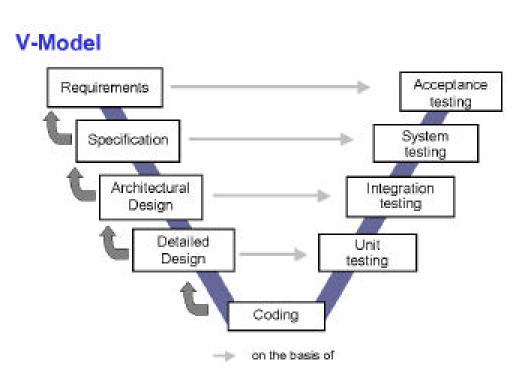
\includegraphics[width=0.5\textwidth]{img/V-model.jpg}
				\caption{Modello a V}
			\end{figure}
	\subsection{Test di validazione}
	\label{sec:5.3}
		I test di validazione servono per accertarsi che il prodotto realizzato sia conforme alle attese di \PROPONENTE. \\
		Per ognuno vengono indicati i passi necessari all'utente per testare i requisiti associati. Il tracciamento tra i test di validazione e i requisiti correlati viene riportato nel documento \ARdoc.
		\subsubsection{TVF1}
			L'utente verifica che possa creare un account. All'utente è richiesto di:
			\begin{enumerate}
				\item registrare un account;
				\item autenticarsi con i dati del proprio account;
			\end{enumerate}
		\subsubsection{TVF1.1}
			L'utente verifica che si possa autenticare. All'utente è richiesto di:
			\begin{enumerate}
				\item inserire un indirizzo email nel campo apposito;
				\item inserire una password nel campo apposito;
				\item confermare i dati inseriti;
				\item verificare di essere autenticato se i dati inseriti sono corretti;
				\item verificare se viene segnalato ogni eventuale errore durante la procedura di autenticazione. 
			\end{enumerate}
		\subsubsection{TVF1.1.5}
			L'utente verifica che ogni eventuale errore riguardante la procedura di autenticazione interrompa la procedura stessa.
			All'utente è richiesto di:
			\begin{enumerate}
				\item verificare se la procedura viene interrotta quando l'indirizzo email inserito non è già stato registrato;
				\item verificare se la procedura viene interrotta quando la password inserita non coincide con quella associata all'indirizzo email inserito;
				\item verificare che ogni errore nell'inserimento dei dati venga segnalato;
				\item verificare di poter cambiare la password qualora non se la ricordasse. 
			\end{enumerate}
		\subsubsection{TVF1.1.5.4}
			L'utente verifica di poter cambiare la password nel caso non se la ricordasse.
			All'utente è richiesto di:
			\begin{enumerate}
				\item inserire l'indirizzo email con cui si è registrato;
				\item verificare di aver ricevuto un'email all'indirizzo inserito con una nuova password casuale;
				\item verificare che la vecchia password del proprio account venga sostituita con quella nuova inviata per email. 
			\end{enumerate}
		\subsubsection{TVF1.2}
			L'utente verifica di poter registrare un nuovo account.
			All'utente è richiesto di:
			\begin{enumerate}
				\item inserire il proprio indirizzo email nell'apposito campo;
				\item inserire uno username nell'apposito campo;
				\item inserire una password nell'apposito campo;
				\item reinserire la password nell'apposito campo;
				\item confermare i dati inseriti;
				\item verificare che l'account venga registrato con i dati inseriti se non ci sono stati errori, e che l'utente venga autenticato automaticamente;
				\item verificare che vengano segnalati gli errori quando ce ne sono.
			\end{enumerate}
		\subsubsection{TVF1.2.7}
			L'utente verifica che vengano segnalati gli errori quando ce ne sono, e di conseguenza venga interrotta la procedura di registrazione.
			All'utente è richiesto di:
			\begin{enumerate}
				\item verificare che venga segnalato un errore quando l'indirizzo email inserito non è corretto, in particolare deve contenere una `@', deve finire con un dominio valido e non deve essere già in uso da un altro utente;
				\item verificare che venga segnalato un errore quando lo username inserito non è corretto, in particolare non deve contenere caratteri non alfanumerici e non deve essere già in uso da un altro utente;
				\item verificare che venga segnalato un errore quando la password inserita non è corretta, in particolare deve essere composta da almeno 6 caratteri e da un massimo di 16;
				\item verificare che venga segnalato un errore quando la password reinserita non concide con quella inserita precedentemente.
			\end{enumerate}
		\subsubsection{TVF2}
			L'utente verifica di poter fare il logout.
		\subsubsection{TVF3}
			L'utente verifica di poter fare un percorso quando è disponibile.
			All'utente è richiesto di:
			\begin{enumerate}
				\item giocare il percorso fino a quando non è concluso;
				\item verificare di poter visualizzare i risultati ottenuti durante l'esecuzione del percorso;
				\item verificare di poter salvare i risultati ottenuti.
			\end{enumerate}
		\subsubsection{TVF3.1}
			L'utente verifica di poter giocare il percorso fino alla sua conclusione.
			All'utente è richiesto di:
			\begin{enumerate}
				\item cercare il beacon corrispondente alla prossima stazione;
				\item giocare la prova relativa a quella stazione.
			\end{enumerate}
		\subsubsection{TVF3.1.1}
			L'utente verifica di poter cercare e trovare il beacon della prossima stazione.
			All'utente è richiesto di:
			\begin{enumerate}
				\item verificare se può cominciare a giocare la prova quando trova il beacon;
				\item verificare se i beacon rilevati ma inutili ai fini della ricerca vengono ignorati dal'app;
				\item verificare di poter chiedere aiuto se non riesce a trovare il beacon o se pensa che ci siano degli errori;
				\item verificare se vengono rilevati dei beacon, esterni al percorso, per segnalare la distanza tra lui e il beacon cercato, e se tale distanza è visualizzata dall'app usando dei valori approssimativi, come dele tacche.
			\end{enumerate}
		\subsubsection{TVF3.1.2}
			L'utente verifica di poter giocare la prova fino alla sua conclusione.
			All'utente è richiesto di:
			\begin{enumerate}
				\item verificare se la prova è una tra quelle previste dall'applicazione;
				\item verificare se vengono visualizzate le istruzioni relative alla prova;
				\item verificare di poter svolgere la prova;
				\item verificare se vengono visualizzati i risultati della prova quando essa viene conclusa;
				\item verificare di poter proseguire il percorso quando la prova giocata non è l'ultima o di poterlo terminare se invece è l'ultima, nel primo caso inoltre l'utente controlla se vengono visualizzate le istruzioni per trovare la stazione successiva.
			\end{enumerate}
		\subsubsection{TVF3.2}
			L'utente verifica di poter visualizzare correttamente i risultati del percorso ottenuti.
			All'utente è richiesto di:
			\begin{enumerate}
				\item verificare se viene visualizzata la durata totale del percorso e se essa viene effettivamente calcolata da quando l'utente accetta di iniziare la prova fino a quando conferma la soluzione dell'ultima prova;
				\item verificare se viene visualizzato il tempo totale impiegato per completare le prove, se esso viene effettivamente calcolato sommando i tempi di ogni prova e se questi ultimi vengono misurati da quando l'utente accetta di iniziare la prova fino alla conferma della sua soluzione;
				\item verificare se viene visualizzato il punteggio totale ottenuto, se esso viene calcolato sommando il punteggio di ogni singola prova, se quest'ultimo viene a sua volta calcolato in base al tipo di prova effettuata e se il risultato ottenuto è il suo nuovo record di quel percorso;
				\item verificare se viene visualizzata la classifica generale relativa a quel percorso e la posizione che l'utente ha raggiunto con quel risultato;
				\item verificare se viene visualizzata la prova con il maggior numero di punti conseguiti;
				\item verificare se viene visualizzata la prova con il minor numero di punti conseguiti.
			\end{enumerate}
		\subsubsection{TVF4}
			L'utente verifica di poter visualizzare le informazioni relative all'app.
			All'utente è richiesto di:
			\begin{enumerate}
				\item verificare di poter visualizzare una schermata con le informazioni generali dell'app;
				\item verificare di poter accedere alla pagina web dell'applicazione tramite un link presente nell'app;
				\item verificare di poter inviare una segnalazione di eventuali errori presenti tramite email.
			\end{enumerate}
		\subsubsection{TVF4.3}
			L'utente verifica di poter giocare la prova fino alla sua conclusione.
			All'utente è richiesto di:
			\begin{enumerate}
				\item verificare se, dopo aver cliccato sul pulsante per le segnalazioni, si apre una nuova email da scrivere tramite il gestore predefinito del dispositivo, dove il destinatario viene impostato automaticamente;
				\item verificare se, dopo aver cliccato il bottone apposito, si apre una schermata dove egli controlla se può selezionare il tipo di errore avuto, verifica se può scegliere la stazione dove pensa si sia presentato l'errore e controlla se, dopo aver confermato i dati, viene inviata un'email all'indirizzo email adibito alle segnalazioni, generata automaticamente in base alle opzioni scelte.
			\end{enumerate}
		\subsubsection{TVF5}
			L'utente verifica di poter visualizzare i risultati dei percorsi effettuati precedentemente.
			All'utente è richiesto di:
			\begin{enumerate}
				\item verificare se, nel caso in cui egli sia autenticato e abbia dei percorsi salvati, viene mostrato l'elenco dei percorsi svolti e se è possibile visualizzare ulteriori informazioni per ognuno di essi;
				\item verificare se, nel caso in cui egli sia autenticato ma non abbia alcun percorso salvato, viene mostrato un invito a svolgere un percorso, oltre ad una spiegazione in cui si informa l'utente che in quella pagina sarà possibile vedere i dati dei percorsi svolti quando verranno salvati;
				\item verificare se, nel caso in cui egli non sia autenticato, viene visualizzato un invito ad autenticarsi, oltre ad una spiegazione dove si informa l'utente che in quella pagina sarà possibile vedere i dati dei percorsi svolti quando verranno salvati.
			\end{enumerate}
		\subsubsection{TVF5.1.1}
			L'utente verifica di poter visualizzare tutte le informazioni relative al percorso salvato scelto.
			All'utente è richiesto di:
			\begin{enumerate}
				\item verificare se viene mostrato il nome del percorso;
				\item verificare se viene visualizzato il nome dell'edificio dove si è svolto il percorso;
				\item verificare se viene mostrata la data in cui si è svolto il percorso;
				\item verificare se viene visualizzato il punteggio totale ottenuto in quel percorso;
				\item verificare se viene mostrato il tempo totale impiegato per poter svolgere il percorso;
				\item verificare se viene visualizzata la posizione attuale nella classifica generale relativa al percorso salvato.
			\end{enumerate}
		\subsubsection{TVF6}
			L'utente verifica di poter visualizzare gli edifici con dei percorsi disponibili più vicini alla sua posizione.
			All'utente è richiesto di:
			\begin{enumerate}
				\item verificare di poter cercare gli edifici inserendo un raggio massimo, oltre a controllare di poter effettivamente visualizzare tutti gli edifici con dei percorsi disponibili nell'area, calcolata in base al valore del raggio immesso, di poter visualizzare informazioni più dettagliate per ognuno di essi e se viene suggerito di aumentare il raggio inserito qualora l'esito della ricerca fosse negativo;
				\item verificare di poter cercare gli edifici decidendo quante strutture mostrare nell'elenco tra quelle più vicine, oltre a controllare che gli edifici elencati siano effettivamente i più vicini e se è possibile visualizzare informazioni più dettagliate per ognuno di essi;
				\item verificare di poter visualizzare tutte le informazioni dell'edificio selezionato.
			\end{enumerate}
		\subsubsection{TVF6.3}
			L'utente verifica di poter visualizzare tutte le informazioni relative all'edificio scelto.
			All'utente è richiesto di:
			\begin{enumerate}
				\item verificare se vengono mostrate le informazioni specifiche dell'edificio;
				\item verificare se viene visualizzato il link alla pagina web dell'edificio;
				\item verificare se vengono mostrati tutti i contatti disponibili per quell'edificio.
			\end{enumerate}
		\subsubsection{TVF6.3.1}
			L'utente verifica di poter visualizzare tutte le informazioni specifiche dell'edificio.
			All'utente è richiesto di:
			\begin{enumerate}
				\item verificare se viene mostrato il nome dell'edificio;
				\item verificare se viene visualizzata la destinazione d'uso della struttura, come ad esempio ``museo di storia egizia'';
				\item verificare se viene mostrato l'indirizzo dell'edificio;
				\item verificare se viene visualizzata una breve descrizione della struttura e del tipo di percorsi presenti.
			\end{enumerate}
		\subsubsection{TVF6.3.3}
			L'utente verifica di poter visualizzare tutti i contatti disponibili dell'edificio.
			All'utente è richiesto di:
			\begin{enumerate}
				\item verificare se viene mostrato il numero di telefono dell'edificio;
				\item verificare se viene visualizzato l'indirizzo email dell'edificio;
				\item verificare se viene mostrato un link alla pagina Facebook dell'edificio nel caso in cui essa esista;
				\item verificare se viene visualizzato un link alla pagina Twitter dell'edificio nel caso in cui essa esista;
				\item verificare se viene mostrato un contatto pubblico di Whatsapp della struttura nel caso in cui esso esista;
				\item verificare se viene visualizzato un contatto pubblico di Telegram della struttura nel caso in cui esso esista.
			\end{enumerate}
		\subsubsection{TVF7}
			L'utente verifica di poter cambiare le proprie credenziali d'accesso.
			All'utente è richiesto di:
			\begin{enumerate}
				\item verificare di poter cambiare la propria password e controllare se essa può effettivamente avere un numero minimo di 6 caratteri e uno massimo di 16;
				\item verificare di poter cambiare il proprio username, di controllare se viene rispettato il vincolo di non poter usare caratteri non alfanumerici per esso e di accertarsi se non è effettivamente possibile utilizzare uno username già in uso da un altro utente;
				\item verificare se l'applicazione informa l'utente quando c'è un errore nei dati inseriti.
			\end{enumerate}
		\subsubsection{TVF8}
			L'utente verifica se viene mostrato un tutorial introduttivo al primo utilizzo dell'app.
		\subsubsection{TVQ1}
			L'utente verifica se viene fornito il manuale per l'utente dell'applicazione.
		\subsubsection{Test di validazione per i requisiti di vincolo} %Se questa sezione viene ritenuta inutile si può pure eliminare
			I requisiti di vincolo rilevati non necessitano di test appositi per motivi diversi:
			\begin{enumerate}
				\item R0V1 è già incluso nella definizione dell'applicazione proposta, inoltre è già verificato nei test dove viene chiesto di controllare se i beacon sono implementati e rilevati correttamente;
				\item R0V2 viene garantito dalla scelta del sistema operativo, visto che Android è specifico per dispositivi mobile.
			\end{enumerate}
	\subsection{Test di sistema}
	\label{sec:5.4}
		I test di sistema servono per accertarsi che il comportamento dinamico del sistema rispetti i requisiti software individuati e descritti nel documento \ARdoc.
		\subsubsection{Descrizione dei test di sistema}
			\begin{tabella}{!{\VRule}l!{\VRule}l!{\VRule}l!{\VRule}l!{\VRule}}
				\intestazionefourcol{Test}{Descrizione}{Stato}{Requisito}
				TSF1 & Viene verificato che il sistema permetta la creazione e la gestione di un account & N.I. & R0F1 \\
				TSF2 & Viene verificato che il sistema permetta la deautenticazione dell'utente & N.I. & R0F2 \\
				TSF3 & Viene verificato che il sistema permetta all'utente di giocare un percorso tra quelli disponibili nel luogo in cui si trova & N.I. & R0F3 \\
				TSF4 & Viene verificato che il sistema permetta all'utente di visualizzare le informazioni dell'app  & N.I. & R0F4 \\
				TSF5 & Viene verificato che il sistema permetta all'utente di visualizzare i risultati dei percorsi effettuati precedentemente & N.I. & R0F5 \\
				TSF6 & Viene verificato che il sistema permetta all'utente di cercare quali sono gli edifici con percorsi più vicini alla sua posizione & N.I. & R0F6 \\
				TSF7 & Viene verificato che il sistema permetta all'utente di modificare le proprie credenziali d'accesso & N.I. & R0F7 \\
				TSF8 & Viene verificato che il sistema permetta all'utente di visualizzare un tutorial introduttivo al primo utilizzo dell'app & N.I. & R2F8 \\
				TSP1 & Viene verificato che in ogni schermata il tempo di latenza per ottenere una risposta dal server sia minore di 5 secondi, a meno che non vi siano problemi di connessione  & N.I. & R0P1 \\
				TSP2 & Viene verificato che il tempo di latenza per cambiare la schermata nell'app sia minore di 0,5 secondi, a meno che non sia richiesta l'interazione con il server & N.I. & R0P2 \\
				TSQ1 & Viene verificato che il codice rispetti le norme e le metriche delle \NPdoc\ e della \hyperref[sec:3.7.3]{Sezione 3.7.3} & N.I. & R0Q1 \\
				TSQ2 & Viene verificato che i documenti rispettino le norme e le metriche delle \NPdoc\ e della \hyperref[sec:3.7.3]{Sezione 3.7.3} & N.I. & R0Q2 \\
				TSQ3 & Viene verificato che venga fornito il manuale perl'utente & N.I. & R0Q3 \\
				
				\hiderowcolors
				\caption{Descrizione dei test di sistema}
			\end{tabella}
	\subsection{Test di integrazione}
	\label{sec:5.5}
		I test di integrazione servono per verificare che tutti i diversi componenti del sistema comunichino correttamente tra loro, e che vi sia all'interno del software il flusso di dati atteso. \\
		Verrà utilizzata una strategia di integrazione incrementale per poter sviluppare e verificare più componenti in parallelo. Questo metodo permette di dare priorità ai test relativi alle componenti che vengono ritenute più importanti e quindi sarà possibile partire dalle componenti che soddisfano i requisiti obbligatori fino ad integrarle con quelle che soddisfano i requisiti opzionali. Inoltre permette di restringere la ricerca dell'errore in caso di test fallito, perché molto probabilmente l'errore si trova nel nuovo componente o dalla sua interazione con il sistema corrente. Non si dovrà escludere il caso in cui il test fallisca perché la nuova istanza di test utilizza un campione di input non trattato in precedenza, portando così il sistema a generare l'errore. \\
		L'integrazione delle parti è bottom-up: innanzitutto verranno inserite le componenti con meno dipendenze funzionali e più funzionalità, cioè che corrispondono ai requisiti obbligatori. Di conseguenza queste componenti saranno testate molte volte in modo da ridurre la possibilità che il prodotto finale contenga difetti, e così si otterrà una versione funzionante nel minor tempo possibile. In seguito si risalirà l'albero delle dipendenze fino all'inserimento delle componenti di alto livello. \\
		Questo metodo è più oneroso rispetto ad altri in quanto richiede che venga generato del codice di supporto, sotto forma di driver e stub, che simuli le componenti mancanti, però permette una maggiore copertura perché testa ripetutamente le componenti più importanti.